\chapter{Planen}\label{ch:planen}
Dieses Kapitel zeigt die in der IPERKA-Phase «Planen» durchgeführten Arbeiten auf. In dieser Phase werden basierend auf den Anforderungen Arbeitspakete definiert und in einem Zeitplan auf die zehn Probe-IPA Tage aufgeteilt. Zudem werden Lösungskonzepte für die Umsetzung der Seite Business Daten erarbeitet und ein Testkonzept erstellt.

\section{Arbeitspakete}
Die gesamte Arbeit der Probe-IPA wird in Arbeitspakete aufgeteilt. Die Arbeitspakete bestehen aus einer zugehörigen Nummer, einem Namen, dem geschätzten Aufwand und einem erwarteten Ergebnis. In dem geschätzten Aufwand sind Zeitreserven mit einberechnet, sodass unvorhergesehenes kompensiert werden kann. Da der Zeitplan in 2-Stunden-Blöcke aufgeteilt ist, wird der geringste Aufwand 2 Stunden sein und im zweier Takt nach oben gehen.

Die Arbeitspakete sind nach der Projektmanagementmethode IPERKA gegliedert. Probe-IPA-spezifische Arbeiten, wie die Expertenbesuche oder das Erstellen des Anhangs, die ausserhalb des eigentlichen Projekts stehen, werden unter «Rahmenaufgaben» aufgeführt.
\subsection{Informieren}
Folgende Arbeitspakete gehören zu der IPERKA-Phase «Informieren».

\begin{longtable}{p{.3\textwidth}|p{.65\textwidth}}
	\hline
	\textbf{Nummer}                 & \textbf{1.1}            \\
	\hline
	\textbf{Name}   				& Projektumfeld analysieren und beschreiben                  \\
	\hline
	\textbf{Geschätzter Aufwand}    & 2h                                    \\
	\hline
	\textbf{Erwartetes Ergebnis}    & Die Aufgabestellung ist beschrieben und für den Lernenden ist der Auftrag klar. Der Lernende kennt das Projektumfeld und hat es dokumentiert.                                    \\
	\hline
\end{longtable}\label{tab:informieren-1.1}

\begin{longtable}{p{.3\textwidth}|p{.65\textwidth}}
	\hline
	\textbf{Nummer}                 & \textbf{1.2}            \\
	\hline
	\textbf{Name}   				& Anforderungen definieren                  \\
	\hline
	\textbf{Geschätzter Aufwand}    & 2h                                    \\
	\hline
	\textbf{Erwartetes Ergebnis}    & Die Anforderungen werden klar definiert und unterteilt in funktionale und nicht funktionale Anforderungen.                                    \\
	\hline
\end{longtable}\label{tab:informieren-1.2}

\subsection{Planen}
Folgende Arbeitspakete gehören zu der IPERKA-Phase «Planen».

\begin{longtable}{p{.3\textwidth}|p{.65\textwidth}}
	\hline
	\textbf{Nummer}                 & \textbf{2.1}            \\
	\hline
	\textbf{Name}   				& Arbeitspakete definieren                  \\
	\hline
	\textbf{Geschätzter Aufwand}    & 4h                                    \\
	\hline
	\textbf{Erwartetes Ergebnis}    & Die gesamten Arbeitspakete sind definiert und nummeriert nach den Phasen von IPERKA.                                    \\
	\hline
\end{longtable}\label{tab:planen-2.1}

\begin{longtable}{p{.3\textwidth}|p{.65\textwidth}}
	\hline
	\textbf{Nummer}                 & \textbf{2.2}            \\
	\hline
	\textbf{Name}   				& Zeitplan erstellen                  \\
	\hline
	\textbf{Geschätzter Aufwand}    & 2h                                    \\
	\hline
	\textbf{Erwartetes Ergebnis}    & Der Zeitplan wird mithilfe der Arbeitspakete erstellt und die bereits erfüllten Aufgaben werden entsprechend markiert.                                    \\
	\hline
\end{longtable}\label{tab:planen-2.2}

\begin{longtable}{p{.3\textwidth}|p{.65\textwidth}}
	\hline
	\textbf{Nummer}                 & \textbf{2.3}            \\
	\hline
	\textbf{Name}   				& Lösungskonzept für die Struktur des Backends                  \\
	\hline
	\textbf{Geschätzter Aufwand}    & 2h                                    \\
	\hline
	\textbf{Erwartetes Ergebnis}    & Ein Lösungskonzept für die Struktur im Backend wird erarbeitet und dokumentiert.                                    \\
	\hline
\end{longtable}\label{tab:planen-2.3}

\begin{longtable}{p{.3\textwidth}|p{.65\textwidth}}
	\hline
	\textbf{Nummer}                 & \textbf{2.4}            \\
	\hline
	\textbf{Name}   				& Lösungskonzept für die Struktur vom Frontend                  \\
	\hline
	\textbf{Geschätzter Aufwand}    & 2h                                    \\
	\hline
	\textbf{Erwartetes Ergebnis}    & Ein Lösungskonzept für die Struktur im Frontend wird erarbeitet und dokumentiert.                                    \\
	\hline
\end{longtable}\label{tab:planen-2.4}

\begin{longtable}{p{.3\textwidth}|p{.65\textwidth}}
	\hline
	\textbf{Nummer}                 & \textbf{2.5}            \\
	\hline
	\textbf{Name}   				& Lösungskonzept für die Struktur von einer Erweiterung                  \\
	\hline
	\textbf{Geschätzter Aufwand}    & 4h                                    \\
	\hline
	\textbf{Erwartetes Ergebnis}    & Der Lernende entscheidet sich zwischen einer der beiden Erweiterungen und erarbeitet für dieses ein Lösungskonzept und dokumentiert diese anschliessend.                                    \\
	\hline
\end{longtable}\label{tab:planen-2.5}

\begin{longtable}{p{.3\textwidth}|p{.65\textwidth}}
	\hline
	\textbf{Nummer}                 & \textbf{2.6}            \\
	\hline
	\textbf{Name}   				& Testkonzept erstellen                  \\
	\hline
	\textbf{Geschätzter Aufwand}    & 4h                                    \\
	\hline
	\textbf{Erwartetes Ergebnis}    & Ein Testkonzept wird erarbeitet. Die zu schreibenden Tests und Testergebnisse sind definiert.                                    \\
	\hline
\end{longtable}\label{tab:planen-2.6}

\subsection{Entscheiden}
Folgende Arbeitspakete gehören zu der IPERKA-Phase «Entscheiden».

\begin{longtable}{p{.3\textwidth}|p{.65\textwidth}}
	\hline
	\textbf{Nummer}                 & \textbf{3.1}            \\
	\hline
	\textbf{Name}   				& Lösungsvarianten evaluieren                  \\
	\hline
	\textbf{Geschätzter Aufwand}    & 4h                                    \\
	\hline
	\textbf{Erwartetes Ergebnis}    & Mögliche Lösungsvarianten wurden evaluiert und die umzusetzende Lösungsvariante ist definiert.                                    \\
	\hline
\end{longtable}\label{tab:entscheiden-3.1}

\subsection{Realisieren}
Folgende Arbeitspakete gehören zu der IPERKA-Phase «Realisieren».

\begin{longtable}{p{.3\textwidth}|p{.65\textwidth}}
	\hline
	\textbf{Nummer}                 & \textbf{4.1}            \\
	\hline
	\textbf{Name}   				& Endpoints für Mindestanforderungen erstellen                  \\
	\hline
	\textbf{Geschätzter Aufwand}    & 4h                                    \\
	\hline
	\textbf{Erwartetes Ergebnis}    & Die Endpoints für die Mindestanforderungen werden erstellt, sodass das Frontend alle Daten, die es braucht, und nur die, die es braucht, bekommt.                                    \\
	\hline
\end{longtable}\label{tab:realisieren-4.1}

\begin{longtable}{p{.3\textwidth}|p{.65\textwidth}}
	\hline
	\textbf{Nummer}                 & \textbf{4.2}            \\
	\hline
	\textbf{Name}   				& Seite und Tabelle im Frontend erstellen                  \\
	\hline
	\textbf{Geschätzter Aufwand}    & 4h                                    \\
	\hline
	\textbf{Erwartetes Ergebnis}    & Die Seite ist mit der entsprechenden URL und im Menü unter Business Daten → Queue-Messages (eingehend) erreichbar. Die Tabelle ist stimmig ins UI eingebaut und entspricht der tabellarischen Darstellung.                                    \\
	\hline
\end{longtable}\label{tab:realisieren-4.2}

\begin{longtable}{p{.3\textwidth}|p{.65\textwidth}}
	\hline
	\textbf{Nummer}                 & \textbf{4.3}            \\
	\hline
	\textbf{Name}   				& Endpoints für Erweiterung erstellen                  \\
	\hline
	\textbf{Geschätzter Aufwand}    & 4h                                    \\
	\hline
	\textbf{Erwartetes Ergebnis}    & Die Endpoints für die Erweiterung werden erstellt, sodass das Frontend alle Daten, die es braucht, und nur die, die es braucht, bekommt.                                    \\
	\hline
\end{longtable}\label{tab:realisieren-4.3}

\begin{longtable}{p{.3\textwidth}|p{.65\textwidth}}
	\hline
	\textbf{Nummer}                 & \textbf{4.4}            \\
	\hline
	\textbf{Name}   				& Erweiterung in die Tabelle integrieren                  \\
	\hline
	\textbf{Geschätzter Aufwand}    & 4h                                    \\
	\hline
	\textbf{Erwartetes Ergebnis}    & Die Erweiterung wird im Frontend in die Tabelle integriert. Das Design der Erweiterung muss stimmig zu der Tabelle und der Seite eingebaut werden.                                    \\
	\hline
\end{longtable}\label{tab:realisieren-4.4}

\begin{longtable}{p{.3\textwidth}|p{.65\textwidth}}
	\hline
	\textbf{Nummer}                 & \textbf{4.5}            \\
	\hline
	\textbf{Name}   				& Release Notes schreiben                  \\
	\hline
	\textbf{Geschätzter Aufwand}    & 1h                                    \\
	\hline
	\textbf{Erwartetes Ergebnis}    & Für die neue Tabelle werden Release Notes geschrieben, um die Tabelle und die Erweiterung zu beschreiben und zu erklären.                                    \\
	\hline
\end{longtable}\label{tab:realisieren-4.5}

\subsection{Kontrollieren}
Folgende Arbeitspakete gehören zu der IPERKA-Phase «Kontrollieren».

\begin{longtable}{p{.3\textwidth}|p{.65\textwidth}}
	\hline
	\textbf{Nummer}                 & \textbf{5.1}            \\
	\hline
	\textbf{Name}   				& Tests                  \\
	\hline
	\textbf{Geschätzter Aufwand}    & 6h                                    \\
	\hline
	\textbf{Erwartetes Ergebnis}    & Das geplante Testkonzept wird umgesetzt und bei Bedarf ergänzt.                                    \\
	\hline
\end{longtable}\label{tab:kontrollieren-5.1}

\begin{longtable}{p{.3\textwidth}|p{.65\textwidth}}
	\hline
	\textbf{Nummer}                 & \textbf{5.2}            \\
	\hline
	\textbf{Name}   				& Codequalität prüfen                  \\
	\hline
	\textbf{Geschätzter Aufwand}    & 2h                                    \\
	\hline
	\textbf{Erwartetes Ergebnis}    & Die Codequalität wird mithilfe der Jenkins-Pipeline überprüft und bei Bedarf überarbeitet.                                    \\
	\hline
\end{longtable}\label{tab:kontrollieren-5.2}

\begin{longtable}{p{.3\textwidth}|p{.65\textwidth}}
	\hline
	\textbf{Nummer}                 & \textbf{5.3}            \\
	\hline
	\textbf{Name}   				& Dokumentation finalisieren                  \\
	\hline
	\textbf{Geschätzter Aufwand}    & 12h                                    \\
	\hline
	\textbf{Erwartetes Ergebnis}    & Die Dokumentation ist nachvollziehbar und verständlich. Das Dokument wird nach Schreibfehlern durchsucht und verbessert, sodass zu diesem Zeitpunkt fast bis gar keine mehr übrig sind. Die Struktur ist einheitlich und Unschönheiten wurden behoben.                                    \\
	\hline
\end{longtable}\label{tab:kontrollieren-5.3}

\subsection{Auswerten}
Folgende Arbeitspakete gehören zu der IPERKA-Phase «Auswerten».

\begin{longtable}{p{.3\textwidth}|p{.65\textwidth}}
	\hline
	\textbf{Nummer}                 & \textbf{6.1}            \\
	\hline
	\textbf{Name}   				& Kurzfassung schreiben                  \\
	\hline
	\textbf{Geschätzter Aufwand}    & 2h                                    \\
	\hline
	\textbf{Erwartetes Ergebnis}    & Das Projekt wird in einer Kurzfassung zusammengefasst.                                    \\
	\hline
\end{longtable}\label{tab:auswerten-6.1}

\begin{longtable}{p{.3\textwidth}|p{.65\textwidth}}
	\hline
	\textbf{Nummer}                 & \textbf{6.2}            \\
	\hline
	\textbf{Name}   				& Reflexion schreiben                  \\
	\hline
	\textbf{Geschätzter Aufwand}    & 2h                                    \\
	\hline
	\textbf{Erwartetes Ergebnis}    & Das Projekt wird vom Lernenden reflektiert und dokumentiert.                                    \\
	\hline
\end{longtable}\label{tab:auswerten-6.2}

\subsection{Rahmenaufgaben}
Folgende Arbeitspakete gehören zu den Rahmenaufgaben.

\begin{longtable}{p{.3\textwidth}|p{.65\textwidth}}
	\hline
	\textbf{Nummer}                 & \textbf{7.1}            \\
	\hline
	\textbf{Name}   				& Projektstruktur aufsetzen                  \\
	\hline
	\textbf{Geschätzter Aufwand}    & 2h                                    \\
	\hline
	\textbf{Erwartetes Ergebnis}    & Aufbau des Gerüstes des \LaTeX Berichtes, welches die Titelseite, ein Glossar, das Quellenverzeichnis und ein Abbildungsverzeichnis beinhaltet. Ein Git-Repository wird für die Dokumentation aufgesetzt.                                    \\
	\hline
\end{longtable}\label{tab:auswerten-7.1}

\begin{longtable}{p{.3\textwidth}|p{.65\textwidth}}
	\hline
	\textbf{Nummer}                 & \textbf{7.2}            \\
	\hline
	\textbf{Name}   				& Aufgabenstellung und Rahmenbedingungen beschreiben                  \\
	\hline
	\textbf{Geschätzter Aufwand}    & 2h                                    \\
	\hline
	\textbf{Erwartetes Ergebnis}    & Die Aufgabenstellung und Rahmenbedingungen hat der Lernende verstanden und beschreibt sie nochmals um dies zu bestätigen.                                    \\
	\hline
\end{longtable}\label{tab:rahmenaufgaben-7.2}

\begin{longtable}{p{.3\textwidth}|p{.65\textwidth}}
	\hline
	\textbf{Nummer}                 & \textbf{7.3}            \\
	\hline
	\textbf{Name}   				& Projektmanagementmethoden definieren                  \\
	\hline
	\textbf{Geschätzter Aufwand}    & 2h                                    \\
	\hline
	\textbf{Erwartetes Ergebnis}    & Eine Projektmanagementmethode wird definiert und durch eine andere wird erläutert, warum sie gewählt wird.                                    \\
	\hline
\end{longtable}\label{tab:rahmenaufgaben-7.3}

\begin{longtable}{p{.3\textwidth}|p{.65\textwidth}}
	\hline
	\textbf{Nummer}                 & \textbf{7.4}            \\
	\hline
	\textbf{Name}   				& Expertenbesuche                  \\
	\hline
	\textbf{Geschätzter Aufwand}    & 2h                                    \\
	\hline
	\textbf{Erwartetes Ergebnis}    & Die Expertenbesuche werden erfolgreich geplant und durchgeführt. Wichtige Informationen bezüglich der Besuche werden an passenden Plätzen erwähnt und dokumentiert.                                    \\
	\hline
\end{longtable}\label{tab:rahmenaufgaben-7.4}

\begin{longtable}{p{.3\textwidth}|p{.65\textwidth}}
	\hline
	\textbf{Nummer}                 & \textbf{7.5}            \\
	\hline
	\textbf{Name}   				& Anhang erstellen                  \\
	\hline
	\textbf{Geschätzter Aufwand}    & 4h                                    \\
	\hline
	\textbf{Erwartetes Ergebnis}    & Ein Anhang mit allen gemachten Änderungen am Quellcode ist dokumentiert und klar von dem unveränderten Code unterscheidbar.                                    \\
	\hline
\end{longtable}\label{tab:rahmenaufgaben-7.5}

\newpage

\section{Lösungskonzept für die Struktur vom Backend}
In diesem Abschnitt wird das Lösungskonzept vom Backend für einen Teil der unter \ref{ch:minimalanforderungen} definierten Anforderungen beschrieben.

\subsection{Erstellung der Endpunkte}
Im Backend existieren noch keine Endpunkte für die Message-Queues, um sie im Frontend darzustellen. Deshalb müssen diese neu implementiert werden. Die Endpoints werden in einer Ressource-Klasse erstellt und rufen Funktionen von einer Service-Klasse auf. Die Service-Klasse wird von einem Interface implementiert und die Standardfunktionen, wie «getAll» oder «update», sind so bereits im Interface definiert und müssen nur noch in der Service-Klasse implementiert werden. Der Grund für das Interface ist, dass es für die Service-Klasse und die Mock-Service-Klasse genutzt werden kann und beide Klassen die gleichen Funktionen haben, aber mit einer unterschiedlichen Implementierung.

Der Zugriff auf die Datenbank erfolgt in einer DAO-Klasse. In dieser Klasse werden mithilfe von Funktionen die Daten aus der Datenbank hervorgeholt und bereitgestellt. Diese Funktionen werden anschliessend von der Service-Klasse aufgerufen und werden von einem DAO-Objekt zu einem DTO-Objekt gemappt, um die Daten in ein passendes Objekt zu füllen, welches anschliessend wieder an das Frontend gesendet wird.

\subsubsection{DAO-Klassen}
Eine DAO-Klasse (Data Access Object) wird verwendet, um die CRUD-Operationen (Create, Read, Update, Delete) bereitzustellen, die benötigt werden, um Daten zu verwalten. Sie abstrahiert die Verbindung zur Datenbank, sodass der Code ausserhalb der DAO-Klasse unabhängig von der Datenzugriffstechnologie, in diesem Fall Hibernate, bleibt.

\subsubsection{Klassendiagramm für das Backend}
Hier wird ein Klassendiagramm dargestellt, mit den verschiedenen Klassen und Beziehungen, um das Verständnis der Erstellung der Endpunkte zu vereinfachen. Diese Version muss nicht der Implementierung entsprechen. Es kann sein, dass während der Implementierung Veränderungen auftreten, die nicht in diesem Diagramm dargestellt werden.

\begin{figure}[H]
	\begin{center}
		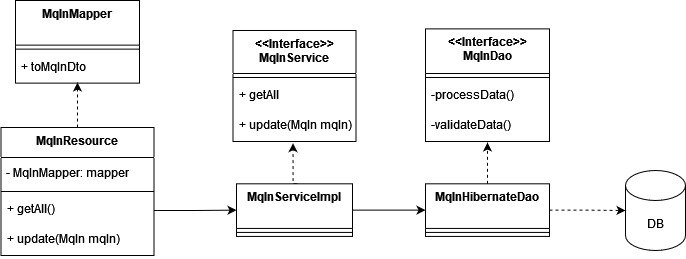
\includegraphics[width=0.8\textwidth]{ressourcen/Klassendiagramm-Backend}
		\caption[Klassendiagramm für das Backend]{Klassendiagramm für das Backend}\label{fig:klassendiagramm-backend}
	\end{center}
\end{figure}

\noindent Der Klassenname ist immer oben in der Box in Bold geschrieben. Die Verbindungen zeigen an, was passiert, wenn ein Endpoint aufgerufen wird. Bei den Interfaces und den dazugehörigen Implementationen ist jeweils nur das Interface beschrieben. Die gestrichelten Verbindungen deuten darauf hin, dass sie diese Klasse implementieren oder sie Gebrauch von einer Funktion in der entsprechenden Klasse machen.

\subsection{Verwendete Technologien}
Um dieses Konzept umzusetzen, werden folgende Technologien verwendet:

\paragraph{Java} ist eine bekannte Programmiersprache und wird in diesem Projekt genutzt, um das Backend zu implementieren.
\paragraph{Hibernate} Hibernate ist ein Framework für Objekt-relationale Abbildung (ORM) in Java, welches ermöglicht, Java-Objekte direkt mit relationalen Datenbanken zu verknüpfen.
\paragraph{Springboot} ist ein Java-Framework, das auf dem Spring-Framework basiert. Es wurde entwickelt, um die Konfiguration und den Aufbau von Anwendungen zu beschleunigen, indem es automatisierte Konfigurationen und eingebettete Server bietet.

\section{Lösungskonzept für die Struktur vom Frontend}
In diesem Abschnitt wird das Lösungskonzept vom Frontende für einen Teil der unter \ref{ch:minimalanforderungen} definierten Anforderungen beschrieben.

\subsection{Bestehende Implementationen}
Im Frontend besteht bereits vieles. Ein Menü muss nicht mehr erstellt werden. Die Seite kann von anderen Implementierungen kopiert und passend zu den Minimalanforderungen gemacht werden. Die Darstellung einer Tabelle im Frontend existiert bereits und muss dadurch nicht erneut implementiert werden. Die Tabelle muss jedoch noch angepasst werden, um die richtigen Spalten anzuzeigen. Durch die bereits existierende Darstellung wird die Tabelle stimmig in das UI eingebaut und wird in etwa gleich aussehen wie die anderen Tabellen im Web-GUI.

\subsection{Neue Implementationen}
Für das Anzeigen der gesamten Nachricht in der Spalte MESSAGE\_SHORT / \_LONG wird ein Knopf im Kontextmenü verwendet. Wenn die gesamte Nachricht angezeigt wird, wird dieser Knopf durch einen anderen ersetzt, welcher die Nachricht wieder auf 50 Zeichen begrenzt.

Ausserdem beinhaltet das Kontextmenü einen weiteren Knopf, um bei einem Eintrag einen neuen Verarbeitungsversuch auszulösen. Dieser Knopf wird bei Einträgen, die bereits in einem Verarbeitungsversuch sind, deaktiviert oder ausgeblendet. Dieser Knopf löst einen Request in das Backend aus, um den neuen Verarbeitungsversuch in der Datenbank zu speichern und ihn auszulösen.

\subsection{Verwendete Technologien}
Um dieses Konzept umzusetzen, werden folgende Technologien verwendet:

\paragraph{TypeScript} ist eine Programmiersprache, die verwendet wird, um die Funktionalitäten für die Tabelle zu implementieren, wie zum Beispiel werden die Requests, an das Backend, mit TypeScript geschrieben.
\paragraph{Angular} ist ein Framework für Single Page Applications (SPAs), bei denen Inhalte dynamisch nachgeladen werden können, ohne dass die Seite neu geladen werden muss. Ausserdem eignet es sich gut, um moderne, skalierbare und performante Webanwendungen zu erstellen.
\paragraph{HTML} (HyperText Markup Language) wird verwendet, um die Struktur und den Inhalt des Webdokuments zu beschreiben. HTML verwendet sogenannte «Tags», die es ermöglichen, Text, Bilder und unter anderem auch Tabellen auf der Webseite anzuzeigen.
\paragraph{CSS} (Cascading Style Sheets) ist eine Stylesheet-Sprache, die das Design und Layout von HTML-Dokumenten festlegt.

\section{Entscheidung der Erweiterung}
Dieser Absatz erklärt den Grund, warum sich der Lernende für eine Erweiterung entschieden hat.

\subsection{Pagination}
Pagination ist etwas Neues für den Lernenden. Er hat es schon öfters gesehen auf anderen Webseiten, hat sich aber noch nie mit der Implementierung auseinandergesetzt. Das Wechseln zwischen mehreren Blättern ermöglicht einen klaren Überblick über die Seite, da die Tabelle durch die Aufteilung eine begrenzte Anzahl Elemente enthält und die Seite durch das nicht überfüllt wirkt. Die Implementierung existiert bereits bei anderen Tabellen und wäre daher nicht allzu schwer, um sie in die Seite einzubauen.

\subsection{Filter}
Die Implementierung für den Filter ist einfacher zu verstehen, weil es Filter auf fast jeder Webseite gibt. Ob versteckt oder sichtbar, kann man sich gut vorstellen, wie das im Hintergrund ablaufen kann. Es gibt mehr Anforderungen für die Erweiterung Filter, aber sie sind einfacher als die bei dem Paginator. Es gibt nur drei Filter-Kriterien, und bei mehreren aktiven Filtern werden sie mit einem «UND» verknüpft.

\subsection{Entscheid}
Die Anforderungen von Pagination sind zwar weniger, aber da sich der Lernende noch nie mit Pagination auseinandergesetzt hat, erschwert es ihm die Implementation und es könnten Fehler auftreten, die viel Zeit kosten. Da die Probe-IPA aber nur 10 Tage zur Verfügung stellt und die Erweiterung Filter schneller gehen könnte, kann der Lernende anschliessend mehr Zeit in die Dokumentation der Erweiterung investieren, um am Ende ein fertiges Produkt zu präsentieren.
\paragraph{Ausgewählte Erweiterung:} Filter

\section{Lösungskonzept für die Struktur vom Filter}
In diesem Abschnitt wird das Lösungskonzept der Erweiterung Filter der unter \ref{ch:erweiterung-filter} definierten Anforderungen beschrieben.

\subsection{Bestehende Implementation}
Im Web-GUI existiert bereits ein Filter unter «Business Daten» → «Fehlgeschlagene Zahlungen». Dieser Filter beinhaltet, wie auch bei der Erweiterung gefordert, einen «Datum von / Datum bis» Filter, welcher kopiert und angepasst werden kann. Für den neuen Endpoint kann auch der bestehende als Beispiel verwendet werden, um die Implementierung zu erleichtern.

Die Filterkriterien und -werte werden auch bereits bei dem Filter auf der Seite «Fehlgeschlagene Zahlungen» in der URL abgebildet. Dadurch kann für die funktionale Anforderung EF6 dies als Beispiel genutzt werden oder sogar teilweise kopiert werden.

\subsection{Neue Implementationen}
Für die zwei anderen Filterkriterien (filtern nach MQ\_IN\_STATUS und Filtern mittels Begriffen im Nachrichteninhalt) gibt es noch keine Implementierung in diesem Projekt, weshalb sie selbst erstellt werden müssen.

\subsubsection{MQ\_IN\_STATUS}
Für diesen Filter wird eine Auswahlliste erstellt mit der folgenden Auswahl:

\paragraph{NEW} Eine neue Nachricht, die bereit für die Bearbeitung ist, für den entsprechenden Job.
\paragraph{STOPPED} Das Bearbeiten der Nachricht wurde gestoppt und wird später weiter bearbeitet.
\paragraph{WAIT} Die Nachricht wurde auf warten gestellt und wird später bearbeitet.
\paragraph{ERROR} Die Nachricht kann nicht wegen eines Fehlers bearbeitet werden und muss manuell bearbeitet werden.
\paragraph{CANCELLED} Der Status kann manuell gesetzt werden zu dem Status STOPPED, um sie vom Löschjob löschen zu lassen.
\paragraph{NOTICED} Der Status kann manuell gesetzt werden zu dem Status ERROR, um sie vom Löschjob löschen zu lassen.
\paragraph{PROCESSED} Die Nachricht wurde erfolgreich bearbeitet.
\paragraph{OUTDATED} Die Nachricht war veraltet, was bedeutet, dass der Job bereits eine neuere Nachricht bearbeitet hat. (z. B. eine Nachricht mit einer höheren Sequenz-Nummer)\newline

\noindent Der ausgewählte Status wird ins Backend geschickt. Die Funktion von diesem Endpoint, welcher den Request bekommt, besteht daraus, eine Anfrage an die Datenbank zu machen. Die Filterung, wie in den Anforderungen \ref{ch:erweiterung-filter} beschrieben, passiert darauf hin direkt auf der Datenbank, um die Performance so wenig wie möglich zu beeinflussen. Würde die Filterung im Backend geschehen, kann das die Performance ein wenig beeinflussen, weshalb es gleich auf der Datenbank gemacht wird. Dies gilt auch für die beiden anderen Filter.

\subsection{Begriffe im Nachrichten Inhalt Filtern}
Dieser Filter wird mithilfe von einem Textfeld erstellt. In dieses Textfeld können Begriffe hineingeschrieben und durch einen Knopf gefiltert werden. Hier wird auch wieder ein Request an das Backend gesendet, um den Nachrichteninhalt von den Elementen in der Datenbank-Tabelle MQ\_TABLE nach diesen Begriffen zu filtern und anschliessend das Ergebnis wieder zurückzusenden an das Frontend.

\subsection{Sequenzdiagramm für die Erweiterung Filter}
In diesem Diagramm wird der Ablauf von einem Filter-Request an das Backend dargestellt. Wegen Zeitgründen werden nicht alle Fälle dargestellt. Sie beruht nur auf einem, zwei und drei Filtern, da alle anderen Möglichkeiten einen ähnlichen Ablauf haben wie die hier dargestellten drei Abläufe.

\begin{figure}[H]
	\begin{center}
		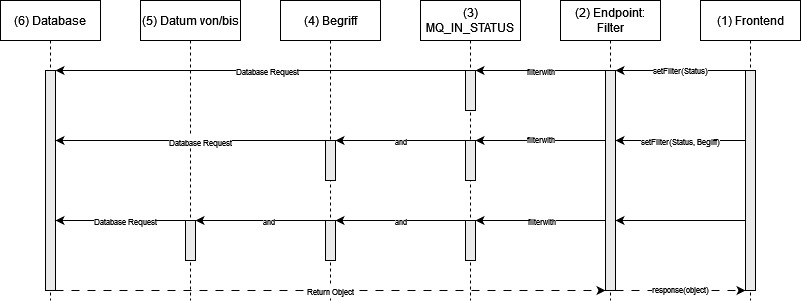
\includegraphics[width=1\textwidth]{ressourcen/Sequenzdiagramm-Erweiterung}
		\caption[Ablauf eines Filter-Request]{Ablauf eines Filter-Request}\label{fig:sequenzdiagramm-erweiterung-filter}
	\end{center}
\end{figure}

Folgende Schritte werden im Sequenzdiagramm durchgeführt.
\begin{enumerate}
	\item Im Frontend wird durch das Auswählen eines Filters ein Request an das Backend gesendet.
	\item Im Backend wird dieser Request angenommen und es wird geprüft, welcher Filter genutzt werden sollte.
	\item Im Fallen von einem Filter wird nichts gross angepasst und eine Anfrage an die Datenbank wird gemacht.
	\item Falls zwei Filter ausgewählt werden, wird eine SQL-Query generiert, die ein AND zwischen beiden Filtern beinhaltet, um nach beidem gleichzeitig zu filtern. Anschliessend wird eine Anfrage an die Datenbank gemacht.
	\item Bei allen drei Filtern wird, ähnlich wie bei zwei Filtern, ein AND zwischen den dreien hinzugefügt und eine Anfrage an das Backend gemacht.
	\item Das erhaltene Resultat von der Datenbank wird dann gemappt und zurück an das Frontend gesendet.
\end{enumerate}

\section{Testkonzept}
Um sicherzustellen, dass die Funktionalität der Implementation fehlerfrei funktioniert und alle Anforderungen richtig eingebunden wurden, wird ein Testkonzept erstellt. Darin befindet sich eine kleine Beschreibung, die Art des Tests, die Vorbedingungen, eine Konfiguration, der Ablauf und das erwartete Resultat.

\subsection{Benötigte Testmittel}
Um die Tests zu implementieren, werden verschiedene Tools und Technologien verwendet. Diese werden hier aufgeführt:

\paragraph{IntelliJ (IDE)} \footnote{\url{https://www.jetbrains.com/de-de/idea/}} ist die Entwicklungsumgebung, in der die Tests geschrieben werden.
\paragraph{Postman} \footnote{\url{https://www.postman.com/}} wird für das manuelle Testen von den Endpointen verwendet.
\paragraph{Mockito} \footnote{\url{https://site.mockito.org/}} wird für das Mocken von Objekten und Klassen verwendet. Mocking ersetzt Objekte und Klassen durch simulierte Versionen, um das erwartete Verhalten nachzuahmen.

\subsection{Automatisierte Tests}
Automatisierte Tests werden nur für die Funktionen im Backend geschrieben. Dies aus dem Grund, weil im Projekt CardX keine Frontend-Tests existieren und diese Implementationen gleich aufgebaut sein sollen wie die anderen Implementationen im Frontend. Sie werden mithilfe von Unit- und Integration-Tests implementiert.

Die Unit-Tests werden für einzelne Funktionen, wie zum Beispiel einen Mapper, verwendet. Sie brauchen keine anderen Systeme und können ohne weiteres ausgeführt werden.

Die Integration-Tests werden oft für Datenbank-Abfragen verwendet, um zu prüfen, ob die Anfrage und das erhaltene Objekt korrekt sind. Diese Art von Testing testet die Zusammenarbeit von verschiedenen Komponenten in einem System, in diesem Fall das Backend und die Datenbank.

\section{Manuelle Tests}
Die manuellen Tests werden für das Backend, mit Postman, und das Frontend durchgeführt. Die neuen Komponenten werden vom Lernenden selbst in einer lokalen Umgebung getestet. Sie werden während der Implementation durchgeführt, um nicht später auf Fehler zu treffen und die Implementation zu vereinfachen.

\section{Testfälle}
Alle automatischen Tests werden auf 25 Einträge limitiert. Sie haben alle den Fehlerzustand MQ\_IN\_STATUS und sind absteigend sortiert nach MODIFIED\_AT. Die erhaltenen Einträge beinhalten nur die Spalten, die vorgegeben sind.

\subsection{Testfälle der Mindestanforderungen}

\begin{longtable}{p{.3\textwidth}|p{.65\textwidth}}
	\hline
	\textbf{Testfall}               & \textbf{M1} \\
	\hline
	\textbf{Beschreibung}   		& Datenbank-Abfrage für die Erstellung von der Tabelle \\
	\hline
	\textbf{Art}    				& Integration-Test \\
	\hline
	\textbf{Vorbedingungen}    		& Das Backend läuft und eine passende Datenbank existiert. \\
	\hline
	\textbf{Konfiguration}   	 	& 
	\begin{itemize}
		\item Die Daten für den Aufruf werden erstellt.
		\item Die erwarteten Daten werden erstellt.
	\end{itemize} \\
	\hline
	\textbf{Ablauf}    				& 
	\begin{enumerate}
		\item Die Datenbank-Abfrage wird durchgeführt.
		\item Die erhaltenen Daten werden mit den bereits erstellten Daten überprüft.
	\end{enumerate} \\
	\hline
	\textbf{Erwartetes Ergebnis}    & Es gibt keine Unterschiede zwischen den Daten aus der Datenbank und den erwarteten Daten.  \\
	\hline
\end{longtable}\label{tab:testfall-M1}

\begin{longtable}{p{.3\textwidth}|p{.65\textwidth}}
	\hline
	\textbf{Testfall}               & \textbf{M2} \\
	\hline
	\textbf{Beschreibung}   		& Neuer Verarbeitungsversuch starten \\
	\hline
	\textbf{Art}    				& Integration-Test \\
	\hline
	\textbf{Vorbedingungen}    		& Das Backend läuft und eine passende Datenbank existiert. \\
	\hline
	\textbf{Konfiguration}   	 	& 
	\begin{itemize}
		\item Die Daten für den Aufruf werden erstellt.
	\end{itemize} \\
	\hline
	\textbf{Ablauf}    				& 
	\begin{enumerate}
		\item Die Datenbank-Abfrage wird durchgeführt.
		\item Die erhaltenen Daten werden überprüft.
	\end{enumerate} \\
	\hline
	\textbf{Erwartetes Ergebnis}    & Ein Objekt auf der Datenbank wurde überschrieben. Das überschriebene Objekt hat einen Status von NEW.  \\
	\hline
\end{longtable}\label{tab:testfall-M2}

\begin{longtable}{p{.3\textwidth}|p{.65\textwidth}}
	\hline
	\textbf{Testfall}               & \textbf{M3} \\
	\hline
	\textbf{Beschreibung}   		& Mapping von DAO zu DTO \\
	\hline
	\textbf{Art}    				& Unit-Test \\
	\hline
	\textbf{Vorbedingungen}    		& Das Backend läuft. \\
	\hline
	\textbf{Konfiguration}   	 	& 
	\begin{itemize}
		\item Ein DAO-Objekt ist erstellt und gefüllt mit Daten.
	\end{itemize} \\
	\hline
	\textbf{Ablauf}    				& 
	\begin{enumerate}
		\item Die Funktion mapDaoToDto() ausführen, mit dem DAO-Objekt als Parameter.
		\item Der erhaltene Wert wird mit dem DAO-Objekt verglichen.
	\end{enumerate} \\
	\hline
	\textbf{Erwartetes Ergebnis}    & Es gibt keine Unterschiede zwischen dem generierten DTO- und dem bereits existierenden DAO-Objekt. \\
	\hline
\end{longtable}\label{tab:testfall-M3}

\begin{longtable}{p{.3\textwidth}|p{.65\textwidth}}
	\hline
	\textbf{Testfall}               & \textbf{M4} \\
	\hline
	\textbf{Beschreibung}   		& Mapping von einer Liste aus DAOs zu einer Liste von DTOs \\
	\hline
	\textbf{Art}    				& Unit-Test \\
	\hline
	\textbf{Vorbedingungen}    		& Das Backend läuft. \\
	\hline
	\textbf{Konfiguration}   	 	& 
	\begin{itemize}
		\item Eine Liste von DAO-Objekten ist erstellt, und die Objekte sind mit Daten gefüllt.
	\end{itemize} \\
	\hline
	\textbf{Ablauf}    				& 
	\begin{enumerate}
		\item Die Funktion listToMqInDto() ausführen, mit der Liste aus DAO-Objekten als Parameter.
		\item Die erhaltenen Werte werden mit der Liste aus DAO-Objekten verglichen.
	\end{enumerate} \\
	\hline
	\textbf{Erwartetes Ergebnis}    & Es gibt keine Unterschiede zwischen den generierten DTO- und den bereits existierenden DAO-Objekten. \\
	\hline
\end{longtable}\label{tab:testfall-M4}


\subsection{Testfälle der Erweiterung Filter}

\begin{longtable}{p{.3\textwidth}|p{.65\textwidth}}
	\hline
	\textbf{Testfall}               & \textbf{M5} \\
	\hline
	\textbf{Beschreibung}   		& Datenbank-Abfrage für das Filtern von einem Filter \\
	\hline
	\textbf{Art}    				& Integration-Test \\
	\hline
	\textbf{Vorbedingungen}    		& Das Backend läuft und eine passende Datenbank existiert. \\
	\hline
	\textbf{Konfiguration}   	 	& 
	\begin{itemize}
		\item Die Daten für den Aufruf werden erstellt.
		\item Der Filter wird gesetzt.
		\item Die erwarteten Daten werden erstellt.
	\end{itemize} \\
	\hline
	\textbf{Ablauf}    				& 
	\begin{enumerate}
		\item Die Datenbank-Abfrage wird durchgeführt.
		\item Die erhaltenen Daten werden mit den bereits erstellten Daten verglichen.
	\end{enumerate} \\
	\hline
	\textbf{Erwartetes Ergebnis}    & Es gibt keine Unterschiede zwischen den gefilterten Daten aus der Datenbank und den erwarteten Daten. \\
	\hline
\end{longtable}\label{tab:testfall-M5}

\begin{longtable}{p{.3\textwidth}|p{.65\textwidth}}
	\hline
	\textbf{Testfall}               & \textbf{M6} \\
	\hline
	\textbf{Beschreibung}   		& Datenbank-Abfrage für das Filtern von mehreren Filtern \\
	\hline
	\textbf{Art}    				& Integration-Test \\
	\hline
	\textbf{Vorbedingungen}    		& Das Backend läuft und eine passende Datenbank existiert. \\
	\hline
	\textbf{Konfiguration}   	 	& 
	\begin{itemize}
		\item Die Daten für den Aufruf werden erstellt.
		\item Die Filter werden gesetzt.
		\item Die erwarteten Daten werden erstellt.
	\end{itemize} \\
	\hline
	\textbf{Ablauf}    				& 
	\begin{enumerate}
		\item Die Datenbank-Abfrage wird durchgeführt.
		\item Die erhaltenen Daten werden mit den bereits erstellten Daten überprüft.
	\end{enumerate} \\
	\hline
	\textbf{Erwartetes Ergebnis}    & Es gibt keine Unterschiede zwischen den gefilterten Daten aus der Datenbank und den erwarteten Daten. \\
	\hline
\end{longtable}\label{tab:testfall-M6}

\begin{longtable}{p{.3\textwidth}|p{.65\textwidth}}
	\hline
	\textbf{Testfall}               & \textbf{M7} \\
	\hline
	\textbf{Beschreibung}   		& Mapping von MqInFilterDto zu MqTableFilterQuery \\
	\hline
	\textbf{Art}    				& Unit-Test \\
	\hline
	\textbf{Vorbedingungen}    		& Das Backend läuft. \\
	\hline
	\textbf{Konfiguration}   	 	& 
	\begin{itemize}
		\item Die Filter werden in einem MqInFilter-Objekt gesetzt.
	\end{itemize} \\
	\hline
	\textbf{Ablauf}    				& 
	\begin{enumerate}
		\item Die Funktion toMqTableFilterQuery() wird ausgeführt mit, den Filtern als Parameter.
		\item Die erhaltenen Daten werden mit den bereits erstellten Filtern überprüft.
	\end{enumerate} \\
	\hline
	\textbf{Erwartetes Ergebnis}    & Es gibt keine Unterschiede zwischen den erstellten und den gemappten Filtern. \\
	\hline
\end{longtable}\label{tab:testfall-M7}

\newpage

\newpage